%**************************************************************
% Capitolo 3 - COSA-COME - Il prodotto dello stage
%**************************************************************
\chapter{Il prodotto\label{cap:ilprodotto}}
\section{Acquisizione delle conoscenze settoriali}
	\subsection{Codifica video}
	Un video digitale è definito come la codifica numerica di un segnale video; la codifica è, dunque, l'azione di trasformare un segnale video in un formato digitale. Questa operazione è effettuata da un software o da un dispositivo elettronico detto codec. Generalmente, i codec eseguono anche compressione lossy, ovvero con perdita di informazioni, in modo tale da ridurre i dati necessari per trasmettere o salvare i flussi video. Esistono anche codec che mantengono inalterata la quantità di informazione; questi vengono definiti lossless.
	\\
	Esistono due famiglie di codec, quelli intraframe e quelli interframe:
	i primi descrivono i frame di un video singolarmente, trattandoli come immagini statiche; i secondi, invece, descrivono i cambiamenti che occorrono tra un fotogramma e l'altro, partendo da frame chiave descritti con codifica intraframe. I codec intraframe risultano, quindi più adatti alla descrizione di scene molto movimentate, senza perdita di qualità, mentre quelli interframe sono più adatti nel caso di sequenze per lo più statiche, per la loro notevole efficienza nel descrivere i pochi cambiamenti avvenuti.

	\subsection{Formati video comunemente usati}
		\subsubsection{M-JPEG}
			Motion JPEG	è un codec video che comprime ogni frame del video originale in una immagine in formato JPEG, un comune formato di compressione con perdita per immagini digitali. Originariamente creato per applicazioni multimediali, M-JPEG è attualmente utilizzato da dispositivi di videoregistrazione come camere digitali, IPcam e webcam.
			\\
			Un grande vantaggio dell'utilizzo di M-JPEG per la codifica video, che ha spinto la sua diffusione sulla maggior parte delle prime fotocamere digitali non professionali, è quello della bassa potenza di calcolo necessaria al suo utilizzo: è sufficiente una modifica software all'encoder hardware per JPEG per poter creare un codec M-JPEG.\@ Inoltre, permette la lettura non lineare del file, utile nel caso di sistemi di video editing. Inoltre l'encoding intraframe che sfrutta limita l'informazione contenuta in ciascun frame M-JPEG a quella di un frame del video originale, permettendo di cambiare velocemente il contenuto, senza considerare i frame precedenti o successivi, come invece accade nelle codifiche interframe come H.264/MPEG-4 AVC.\@
			\\
			Con l'accrescere della potenza di calcolo, M-JPEG	è stato soppiantato da MPEG-4, per la resa qualitativamente molto migliore a parità di bitrate, infatti JPEG è inefficiente nello spazio di archiviazione. Inoltre M-JPEG non sfrutta tecniche di predizione spaziale, come H.264/MPEG-4 AVC, che permetterebbero un ulteriore risparmio di spazio, a discapito di una maggiore potenza di calcolo necessaria.

		\subsubsection{MPEG-1}
			MPEG-1 è uno standard per la compressione con perdita di video e audio progettato per comprimere video con la qualità variabile tra il video di una \gls{VHS} e l'audio di un CD fino a 1.5Mbit/s senza perdita di qualità eccessive, permettendo la creazione di video CD, trasmissioni TV via satellite e via cavo e \gls{DAB}. Attualmente, MPEG-1 è il formato lossy con più supporto di compatibilità al mondo e uno degli standard che ha introdotto più noti è stato il formato audio MP3.
			\\
			MPEG-1 introduce molte tecnologie, frutto di studi statistici, che gli permettono di risparmiare molti dati per descrivere lo stesso video con poca perdita di qualità: innanzitutto l'utilizzo della trasformata DCT su blocchi di \(8\cdot8\) permette di ottenere coefficienti tra loro incorrelati e solo alcuni di questi sono dominanti, permettendo un alto livello di compressione. I coefficienti DCT ottenuti vengono quantizzati, con una grana più fine nelle frequenze più basse e con una più grossa nelle frequenze più alte. Queste influiscono meno sul risultato finale e il loro annullamento permette di diminuire il bitrate complessivo senza pesanti perdite di qualità.
			Data la grande quantità di zeri dovuti alla quantizzazione, si utilizza una codifica run-length, ovvero si indicano i valori a coppie (a, b), dove a rappresenta il valore di un coefficiente non nullo e b il numero di zeri che lo precedono. Si sfrutta infine una codifica entropica basata su una tabella di valori standardizzati, ottenuti con un approccio basato sulla codifica di Huffman.

		\subsubsection{MPEG-4}
			MPEG-4 è basato sugli standard MPEG-1, MPEG-2 e QuickTime. Si è osservato che, in caso di video con sezioni statiche o relativamente statiche, molti frame sono riproducibili dai precedenti. È stata, quindi, realizzata una tecnica che sfrutta la somiglianza tra frame vicini per risparmiare spazio nella codifica. Questa si ottiene indicando alcuni frame come frame chiave (I-Frame) e generando i frame seguenti come trasformazioni del frame principale
			\\
			MPEG-4 permette di creare oggetti multimediali con migliori capacità di adattamento e flessibilità, in grado di migliorare la qualità del risultato finale; inoltre è in grado di adattare la propria qualità sia a stream a basso bitrate, anche 1 Mbit/s, fino a formati ad alta risoluzione, come 4K e 8K.
			\\
			Le sue ottime performance di qualità e compressione costano in potenza computazionale, a causa della complessità della fase di quantizzazione; al contrario, la decodifica per la riproduzione è sufficientemente rapida e poco costosa, grazie anche a decodificatori hardware specializzati, ormai comunemente integrati nella maggior parte dei processori.

		\subsubsection{WebM}
			WebM è un formato video royalty-free pensato per il web, rilasciato sotto licenza BSD, il cui sviluppo è sponsorizzato da Google. WebM sfrutta il motore di codifica VP9 e audio Opus ed è supportato nativamente dai maggiori browser, inclusi dispositivi mobile. WebM punta ad una migliore efficienza di compressione rispetto a MPEG-4 e sta sostituendo GIF come formato di animazione video. Mentre il formato è libero, i motori VP8 e VP9 sono patentati Google e solo nel 2013 MPEG LA ha raggiunto un accordo con la multinazionale per la licenza delle componenti essenziali all'implementazione dei codec. Le attuali implementazioni libere (libvpx) mostrano un significativo vantaggio nei tempi di codifica e nel risparmio di bitrate rispetto a MPEG-4 H.264 e H.265.
	\subsection{Protocolli}
	Un protocollo di rete è un protocollo di comunicazione utilizzato da in una rete informatica: la definizione formale a priori delle modalità di interazione tra due o più apparecchiature elettroniche devono utilizzare per poter comunicare tra di loro tramite una rete.

		\subsubsection{Protocolli per il video streaming}
			Quando parliamo di protocolli di rete possiamo dividerli due categorie in base al tipo di trasmissione che utilizzano, ovvero se stream-oriented o message-oriented. Questa differenza, riscontrata al Transport Layer della pila OSI, è la base dei due più famosi protocolli di quel livello: TCP e UDP.\@
			\begin{figure}[H]
				\begin{center}
					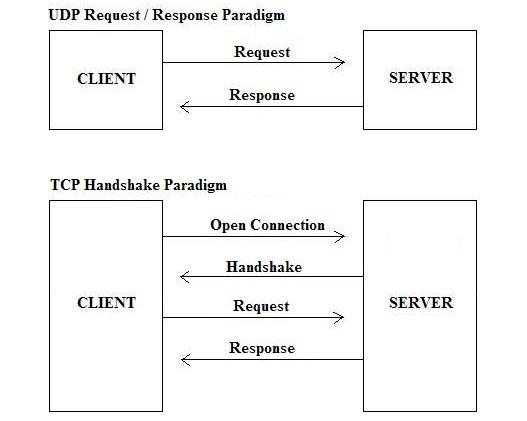
\includegraphics[width=16.5cm,height=8cm,keepaspectratio]{immagini/tcp-udp-connections}	
					\caption[Schema di connessione di TCP e UDP]{Schema di connessione di TCP e UDP
					\\
					Source: Wikimedia commons, Khandarmaa, CC BY-SA}
				\end{center}
			\end{figure}
			TCP (Transmission Control Protocol) appartiene alla prima categoria: provvede alla realizzazione dei una connessione affidabile, nella quale i dati vengono suddivisi in pacchetti ordinati e in caso di errori di trasmissione il ricevente può richiederne il reinvio. Questo protocollo è pensato per la consistenza dei dati e assicura che le informazioni richieste arrivino tutte, integre e nell'ordine corretto al ricevente.
			\\
			UDP (User Datagram Protocol), al contrario, appartiene al secondo genere: utilizza un modello connectionless, pensato per messaggi atomici, e non garantisce che l'ordine di invio di un certo numero di pacchetti sia lo stesso con il quale vengono ricevuti. Inoltre, il protocollo non ha particolari misure di prevenzione della corruzione dei dati, se non un checksum dei contenuti del pacchetto, che ne permette la verifica di integrità.
			\\
			Nel caso di applicazioni di streaming è importante nominare anche il protocollo SCTP (Stream Control Transmission Protocol): si tratta di un protocollo message-oriented e connectionless, simile a UDP, ma che aggiunge alcune feature di TCP, come l'ordinamento dei pacchetti e la richiesta di reinvio. Questo permette al ricevente di mantenere la coerenza dei dati, anche in caso di messaggi lunghi, e di ricevere più stream di pacchetti in parallelo.

		\subsubsection{Tipologie di streaming}
			Nel caso applicativo dello streaming video si riscontrano due possibili situazioni:
			nel caso di streaming real-time l'obiettivo è quello di trasmettere un video con una latenza molto bassa, anche a discapito della qualità video; si pensi, ad esempio, quanto è negativa l'esperienza di un utente che durante una videoconferenza si accorge che un altro utente deve aspettare del tempo prima di ricevere la propria registrazione.
			\\
			Altro caso è quello dello streaming on-demand, nel quale un utente richiede l'accesso ad una risorsa video remota e la sua visualizzazione deve essere riportata con la qualità nativa; in questo caso l'utente è disposto ad aspettare qualche secondo di precaricamento iniziale, ma risulta particolarmente infastidito dalle interruzioni, magari a causa del buffering.
			\\
			Nel primo caso il protocollo ideale è quello che trasmette con il bitrate più alto possibile e con la massima frequenza di invio di messaggi; infatti il solo bitrate non basta, una frequenza di invio alta permette di limitare la latenza alla sorgente del segnale, rimpicciolendo il tempo di attesa tra un intervallo e il successivo. Per questo tipo di trasmissioni il protocollo il protocollo più adatto è UDP, per la dimensione variabile del messaggio, la piccola dimensione del suo header e l'assenza di garanzie di consistenza non fondamentali, come la certezza che tutti i dati siano stati ricevuti. Sono nati quindi numerosi protocolli per l'Application Layer OSI basati su UDP, adattati alla trasmissione di streaming video, come RTP, RTSP, RTMP.\@ A questo tipo di protocolli vengono spesso associati protocolli di controllo, come RTMCP e RRCP, che permettono a trasmittente e ricevente di accordarsi sul formato dei dati e sul bitrate da utilizzare.
			\\
			Nel secondo caso il protocollo deve garantire la consistenza e l'integrità della trasmissione, pur mantenendo un bitrate elevato. Questo tipo di trasmissione può essere ottenuta tramite un protocollo stream-oriented, come quello di TCP.\@ Nascono, quindi, anche nel caso di TCP protocolli per l'Application Layer OSI progettati per stream di video, come MPEG-DASH (Dynamic Adaptive Streaming over HTTP), HLS (HTTP Live Streaming) di Apple e Microsoft Smooth Streaming. Per risolvere il problema delle interruzioni, molti servizi lasciano al client la possibilità di caricare dinamicamente più di una versione dello stesso contenuto, in base alla disponibilità di bandwidth.
			\\
			Esiste infine un ulteriore funzionalità che sta diventando comune nei servizi più grandi: quella dello streaming ibrido. Il servizio si basa su streaming real-time, ma permette agli utenti di rivedere una scena già trasmessa, comportandosi come uno streaming on-demand. Questo tipo di servizio richiede che il contenuto registrato venga salvato e velocemente diffuso all'interno della piattaforma, per poi essere reso disponibile, come per i restanti contenuti on-demand.

		\subsubsection{UDP e i problemi di firewall}
			Sebbene i protocolli basati su UDP siano particolarmente adatti alle comunicazioni real-time, soffrono di un grave problema legato alle regole applicate ai firewall, specialmente nel caso di reti pubbliche o aziendali: capita molto spesso che per evitare minacce proveniente da reti esterne gli amministratori decidano di bloccare tutti, o quasi, i pacchetti UDP in entrata, a meno di risposta ad una chiamata proveniente dall'interno. Questa pratica è diventata molto comune, tanto che anche servizi di streaming, come YouTube e Twitch, o di telecomunicazione, come Skype o Hangouts, siano stati costretti ad incapsulare il contenuto dei propri pacchetti UDP in pacchetti TCP, per superare le protezioni e offrire i propri servizi.

		\subsubsection{WebRTC}
			%TODO: schema e spiegazione del funzionamento
			WebRTC è un insieme di protocolli di rete che permettono l'invio di messaggi in real-time tramite connessioni peer-to-peer. Il sistema è pensato per essere integrato nativamente nei browser, in modo tale da poter essere utilizzato, tramite un'interfaccia, da webapp apposite per comunicare con componenti di backend e browser di altri utenti. WebRTC sfrutta il protocollo RTP, per il trasferimento di audio e video, e lo stato attuale del suo supporto da parte dei principali browser è quasi totale: solo vecchie versioni di Internet Explorer e Safari non lo supportano. Sebbene questa tecnologia sia standardizzata e il suo impiego sia sempre più frequente da parte di servizi di videochat, le sue implementazioni per le piattaforme Android e iOS sono ancora acerbe e poco documentate; per questo motivo è ancora comune definire un protocollo di comunicazione specifico per l'applicazione, piuttosto di utilizzare questo standard.

	\subsection{Architettura di una piattaforma di streaming}
		\subsubsection{Struttura di massima}
			Una piattaforma di video streaming si compone di cinque elementi principali:
			\begin{itemize}
			\item La rete di inbound, ovvero il sistema di reti che gestisce l'ingresso di dati nella piattaforma, siano questi file video o stream;
			\item Il motore di codifica, che permette di ricodificare i video in ingresso per renderli disponibili nei formati opportuni ai passaggi successivi.
			\item Il sistema di storage, per il salvataggio dei contenuti per la breve, media e lunga conservazione;
			\item Il sistema di gestione e ricerca dei contenuti, che permette agli utenti di caricare, cercare e riprodurre i contenuti di proprio interesse;
			\item Il sistema di distribuzione dei contenuti, ovvero la rete che si occupa della trasmissione di dati ai client.
			\end{itemize}

			\begin{figure}[H]
				\begin{center}
					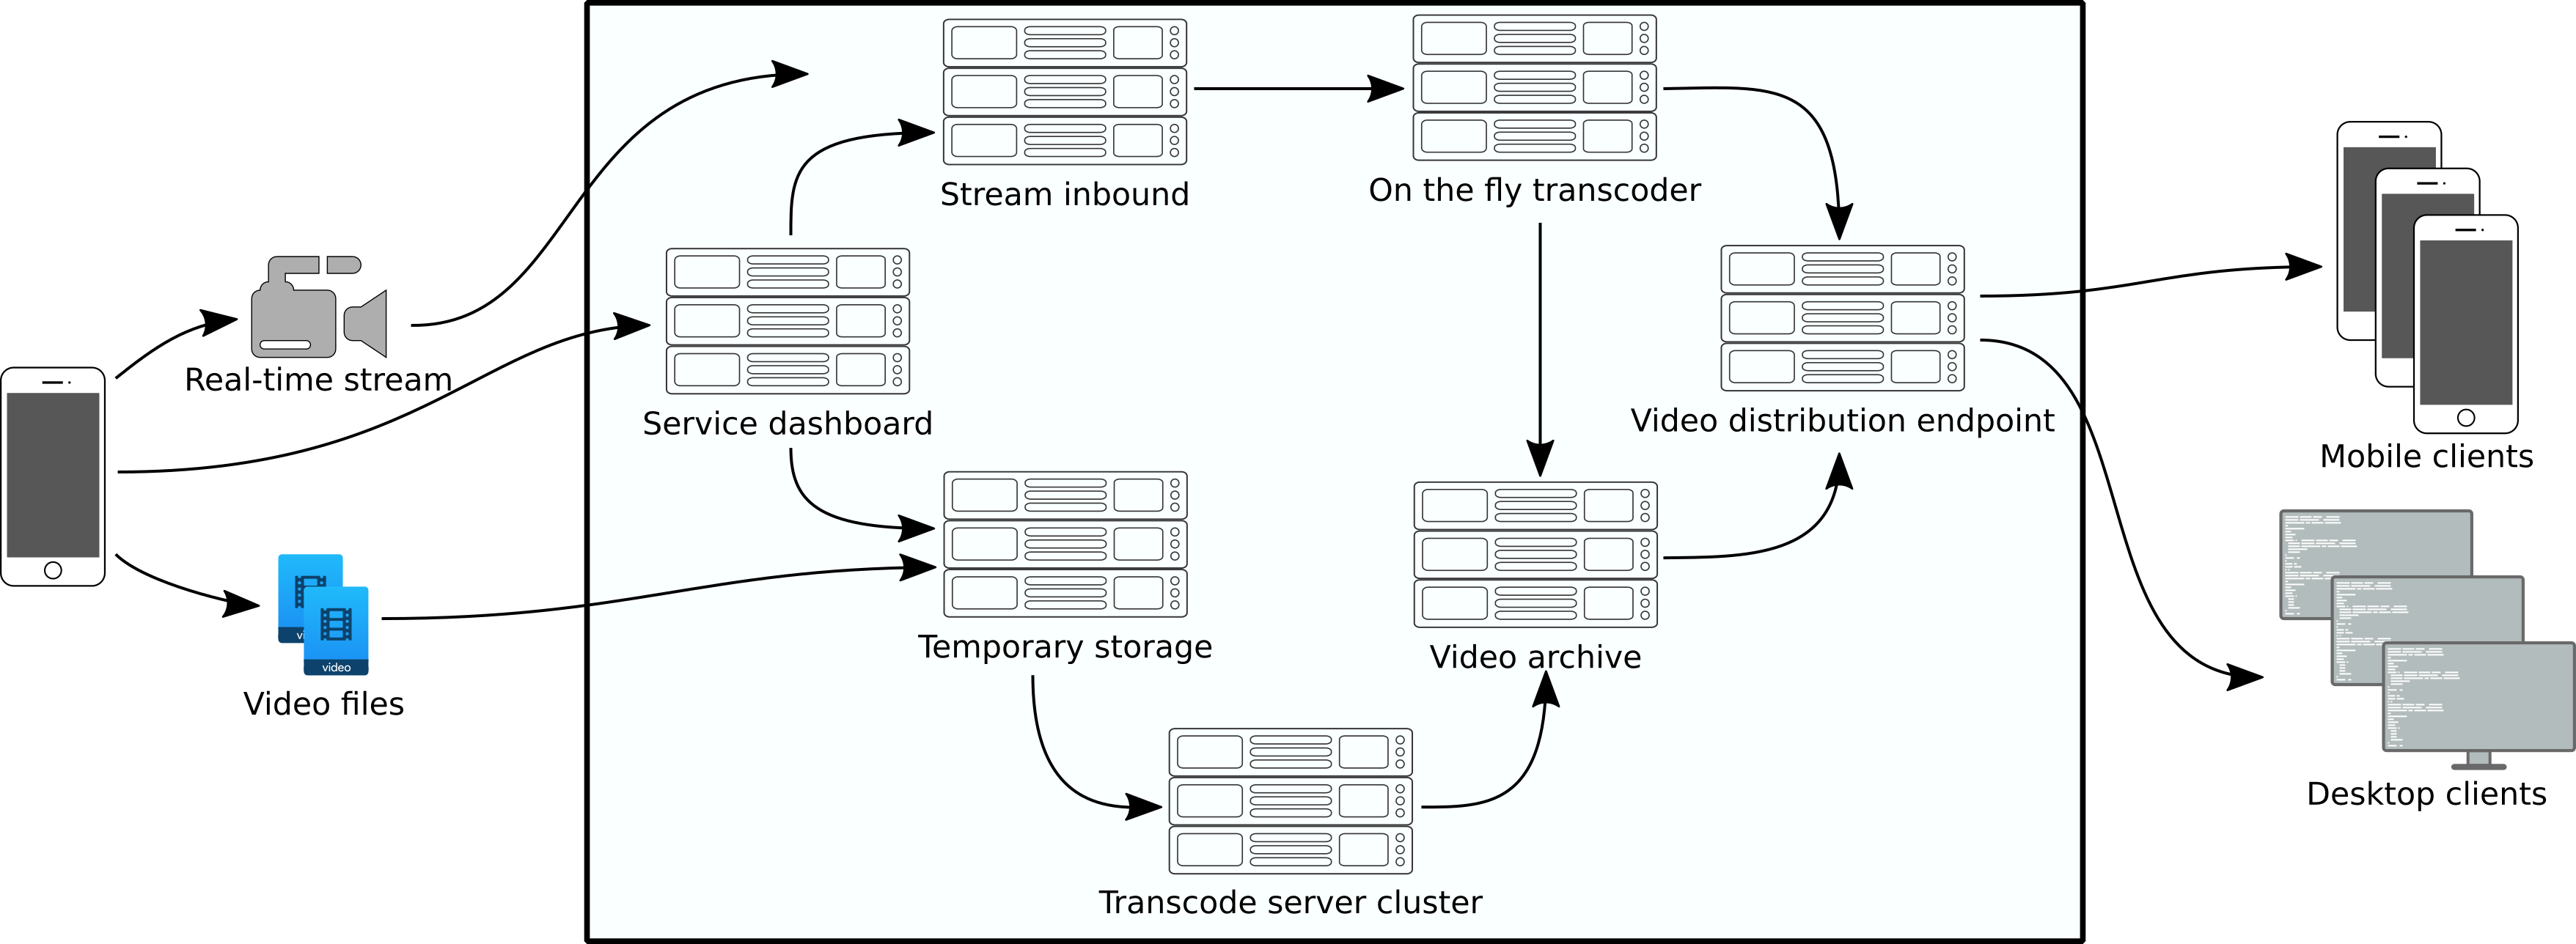
\includegraphics[width=16.5cm,keepaspectratio]{immagini/schema-architettura-piattaforma-streaming}
					\caption{Schema generale di una piattaforma di streaming}
				\end{center}
			\end{figure}

		\subsubsection{Inbound e transcodifica}
			La rete di inbound è la parte del sistema che si occupa di accettare file e stream da parte degli utenti e di inoltrarli ai nodi sottostanti. Questa componente è soggetta ai tipici problemi delle applicazioni web con un numero di utenti rilevante, ovvero la stabilità del servizio, la necessità di reti ad alta disponibilità, il bilanciamento del carico di lavoro tra i nodi sottostanti.
			\\
			I contenuti caricati tramite il sistema di inbound vengono, poi, inviati ai motori di codifica, componenti specializzati nell'encoding dei video. A seconda del tipo di input è possibile scegliere se utilizzare un transcodificatore per lo streaming, in grado di rielaborare il formato video di uno stream ``al volo'' e con poca latenza aggiuntiva, oppure, nel caso di file video, questi vengono caricati in storage temporanei e successivamente elaborati da transcodificatori comuni.

		\subsubsection{Storage e organizzazione dei contenuti}
			%TODO: espandere
			Il sistema di storage si occupa dell'organizzazione dei contenuti, del loro salvataggio e del loro recupero. Al semplice filesystem viene associato un database, spesso non relazionale, per la gestione di metadati, testi, commenti e dati aggiuntivi. Il sistema deve permettere una veloce ed efficace ricerca dei contenuti, per permettere agli utenti di accedere alle informazioni volute.

		\subsubsection{Outbound, protocolli e \gls{CDN}}
			Nel caso della distribuzione di contenuti verso i client sono generalmente utilizzati protocolli basati su TCP, come MPEG-DASH, Apple HLS e Microsoft Smooth Streaming. Questo tipo di protocolli permettono più stream paralleli e la possibilità di eseguire caching dei contenuti trasmessi, particolarmente utili nel caso di utilizzo di \gls{CDN} per estendere la distribuzione. Queste reti, solitamente di proprietà delle aziende di telecomunicazione su cui poggiano gli ISP, offrono un servizio di caching che permette di spostare il carico di rete dovuto all'accesso ai contenuti dai server principali del servizio a server più piccoli e dislocati sul territorio. Questo tipo di distribuzione, non solo diminuisce il carico di rete, limitato quindi alla sola autorizzazione all'accesso, ma permette di avere latenza e tempi di caricamento minori da parte degli utenti.			

		\subsubsection{Message relay}
			Esistono casi di servizi di streaming che devono permettere il reinvio di dati tra due client, senza alcuna modifica ai contenuti trasmessi; in questo caso di parla di message relay. Questo tipo di servizio è fondamentale se i due client non possono comunicare direttamente, magari perché bloccati da firewall o nascosti da una rete con NAT.\@

		\subsubsection{Servizi annessi}
			Molte piattaforme di streaming non si limitano alla sola trasmissione di contenenti ma offrono anche un certo numero di servizi annessi. In particolare le informazioni legate alla demografia degli utenti e alla loro profilazione sono di particolare interesse per i creatori. Inoltre sono comuni servizi di monetizzazione e annunci pubblicitari, cifratura dei contenuti e sistemi DRM.\@


	\subsection{Trasmissione dei contenuti in mobilità}
			%TODO: aggiungere alla bibliografia http://www.telegraph.co.uk/technology/2016/11/01/mobile-web-usage-overtakes-desktop-for-first-time/
			La quantità di utenti che consumano contenuti multimediali su applicazioni mobile sempre più in aumento, tanto che nel Novembre 2016 si è registrato il sorpasso della quantità di utenti su tali piattaforme, rispetto ai desktop. È in crescita anche l'utilizzo di questi dispositivi per eseguire live stream, specialmente legati a social network, come Twitter, Facebook e Google+.
			L'utilizzo di dispositivi mobile aggiunge un ulteriore strato di complessità alla comunicazione con i servizi web, come anche le piattaforme di streaming.
			Le difficoltà maggiori che si incontrano in questo campo sono la limitata potenza computazionale dei dispositivi e autonomia energetica, i limiti imposti da una rete senza fili e la grande frammentazione dei sistemi, specialmente quando si tratta di Android.
			La maggior parte dei problemi precedentemente citati viene gestito dal sistema operativo, ma restano le limitazioni fisiche, ovvero la velocità di trasferimento dei dati:
	\subsection{Reti per dispositivi mobile}
			Le principali reti disponibili per dispositivi mobile possono essere riassunte nelle seguenti:
		\subsubsection{4G --- LTE}
			LTE, lo standard commerciale 4G per le telecomunicazioni mobile, supporta downlink con velocità di picco di 300 Mbit/s e uplink di 75 Mbit/s in caso di posizione statica. Questo tipo di connessione è ampiamente sufficiente alla trasmissione di video in alta risoluzione e alto framerate. LTE ha lo svantaggio di essere soggetto a forti interferenze quando deve attraversare materiali solidi come muri o persone.
		\subsubsection{Wi-Fi}
			L'ultimo standard Wi-Fi, IEE 802.11ac, ormai comunemente supportato dai dispositivi mobile in commercio, raggiunge una velocità di trasmissione di circa un Gbit/s. Il precedente standard, IEE 802.11n, era limitato a 300 Mbit/s tramite l'utilizzo di sistemi ad antenna multipla. Anche Wi-Fi è soggetto ad interferenze, specialmente quando utilizzato sulle frequenze più alte, a 5GHz. Oltre alla comune connessione a infrastruttura, IEE 802.11 supporta anche connessioni peer-to-peer tramite il protocollo Wi-Fi Direct, che riduce i consumi e massimizza il throughput.
		\subsubsection{Bluetooth}
			Bluetooth 5 ha un throughput molto più basso dei precedenti canali di comunicazione; raggiunge, infatti, circa 50 Mbit/s, un bitrate appena sufficiente alla trasmissione di video HD, al contrario, però, la distanza tra il trasmittente e il ricevente è molto più ridotto. Il vantaggio principale di Bluetooth è quello di utilizzare una minore quantità di energia elettrica per comunicare con altri dispositivi.

\section{Analisi dei requisiti}
	\subsection{Analisi preliminare}
		L'analisi preliminare si è focalizzata sulla definizione degli attori e degli obiettivi e delle funzionalità principali del software da produrre.
		\\
		Il software deve gestire l'autenticazione di amministratori e utenti; questi hanno, in entrambi i casi, hanno un'identità univoca e un token di accesso. Gli amministratori hanno la possibilità di creare e rimuovere canali, aggiungere e togliere utenti e gestirne l'autenticazione.
		Gli utenti possono autenticarsi, inviare messaggi nei canali dove sono registrati o abbandonarne uno.
		\\
		Ho definito, in collaborazione con gli sviluppatori del team che si occupa del progetto, gli attori del sistema, le interazioni che possono intraprendere e i risultati di ciascuna di queste. Per fare ciò ho definito i casi d'uso tramite un diagramma UML.\@

	\subsection{Definizione dei casi d'uso}
		Segue una versione ristretta della definizione dei casi d'uso definiti.
		\begin{figure}[H]
			\begin{center}
			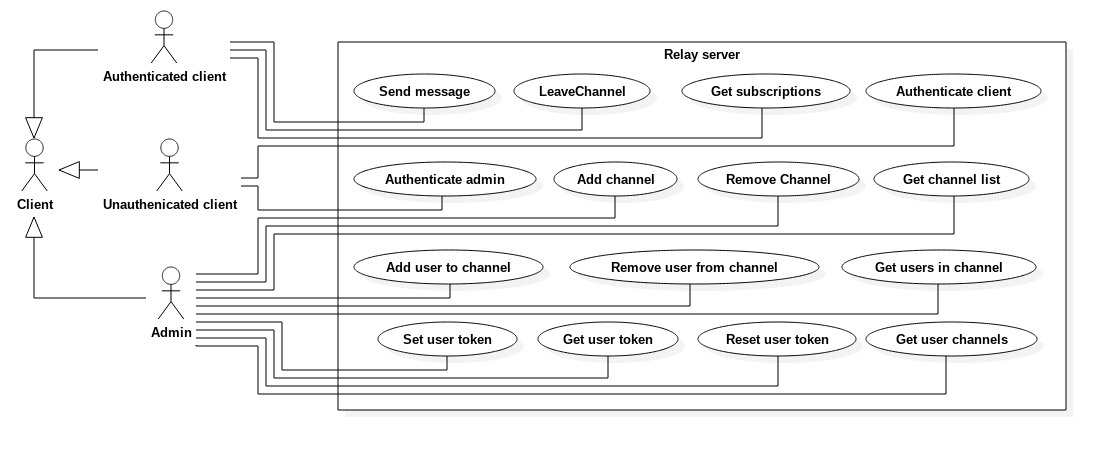
\includegraphics[width=16.5cm,keepaspectratio]{UML/png/Use Case Model__Use Cases_0}
			\caption{Diagramma dei casi d'uso del sistema}
			\end{center}
		\end{figure}

		\subsubsection{Attori}
		\begin{itemize}
			\item \textbf{Client}: un utente che interagisce con il sistema;
			\item \textbf{Unauthenticated Client}: un client non ancora autenticato;
			\item \textbf{Authenticated Client}: un client che ha eseguito l'autenticazione ed è registrato all'interno di almeno un canale;
			\item \textbf{Admin}: un utente o un sistema automatico che ha il ruolo di amministratore del servizio offerto dal server.
		\end{itemize}

		\subsubsection{Casi d'uso di Unauthenticated Client}
		\begin{itemize}
			\item \textbf{Authenticate client}: L'utente esegue l'autenticazione su sistema come client;
			\item \textbf{Authenticate admin}: L'utente esegue l'autenticazione su sistema come admin.
		\end{itemize}

		\subsubsection{Casi d'uso di Authenticated Client}
		\begin{itemize}
			\item \textbf{Send message}: L'utente invia un messaggio all'interno di un canale in cui è registrato; 
			\item \textbf{Leave channel}: L'utente lascia il canale e viene deregistrato; 
			\item \textbf{Get subscriptions}: L'utente ottiene la lista dei canali nei quali è registrato; 
		\end{itemize}

		\subsubsection{Casi d'uso di Admin}
		\begin{itemize}
			\item \textbf{Add channel}: L'Amministratore crea un nuovo canale;
			\item \textbf{Remove channel}: L'amministratore elimina un canale;
			\item \textbf{Get channel list}: L'amministratore ottiene la lista dei canali registrati;
			\item \textbf{Add user to channel}: L'amministratore registra un utente in un certo canale;
			\item \textbf{Remove user from channel}: L'amministratore rimuove un utente da un canale;
			\item \textbf{Get users in channel}: L'amministratore ottiene la lista degli utenti registrati in un canale;
			\item \textbf{Set user token}: L'amministratore imposta il token di autenticazione di un utente;
			\item \textbf{Get user token}: L'amministratore ottiene il token di autenticazione di un utente;
			\item \textbf{Reset user token}: L'amministratore resetta il token di autenticazione di un utente;
			\item \textbf{Get user channels}: L'amministratore ottiene la lista dei canali in cui un certo utente è registrato.
		\end{itemize}
		

\section{Struttura della piattaforma}
Una volta definiti i casi d'uso, ho proceduto alla scelta dei protocolli di rete da utilizzare e la progettazione strutturale del sistema.
	\subsection{Protocolli}
	Ho eseguito la scelta dei protocolli in collaborazione con il team di sviluppatori che lavorava sul client Android, per trovare la migliore soluzione in termini di latenza, throughput e complessità di implementazione.
	\\
	I protocolli UDP sono stati scartati a causa dei problemi con firewall riportati precedentemente.
	Le specifiche del servizio richiedono che sia possibile inviare messaggi di qualsiasi tipo, sia atomici, sia stream di dati. Per semplificare l'invio di dati generici, senza essere necessariamente legati ad un certo protocollo dello strato applicativo, abbiamo deciso di utilizzare dei WebSocket ed esistono implementazioni open-source dello standard per la maggior parte delle piattaforme, inclusi iOS e Android e Java, rendendo, quindi, l'implementazione di client e server più semplice.
	
	\subsection{Diagramma strutturale}
	Segue in Fig.~\ref{diagrammaclassi} il diagramma UML delle classi semplificato.

	\begin{figure}[H]
		\begin{center}
			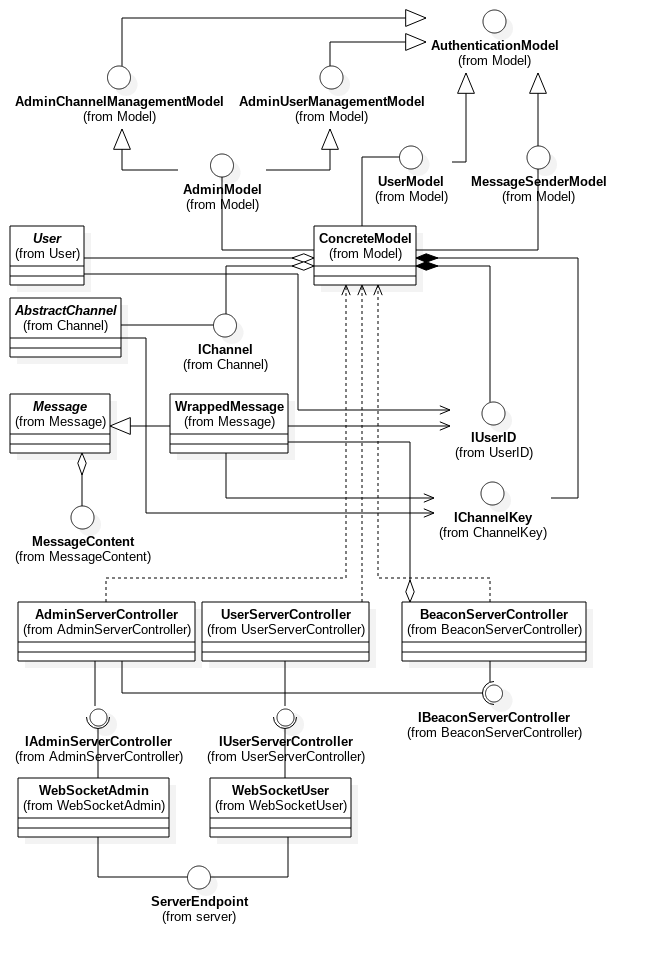
\includegraphics[height=18.5cm,keepaspectratio]{UML/png/Design Model__SimpleClasses_6}
			\caption{Diagramma delle classi del sistema}\label{diagrammaclassi}
		\end{center}
	\end{figure}

		\subsubsection{ConcreteModel e interfacce del modello}
	Il modello è responsabile del salvataggio e della gestione delle informazioni legate agli utenti, ai canali, alle registrazioni e ai messaggi da inviare. Per organizzare chiaramente le sue funzionalità ho utilizzato interfacce molto specifiche.

		\subsubsection{IUserID e IChannelKey}
	Per identificare univocamente un utente o un canale ho designato due interfacce per due classi di oggetti che permettono di ottenere un identificativo univoco sotto forma di stringa; in questo modo è possibile referenziare uno di questi oggetti indicandone il solo ID

		\subsubsection{User}
	La classe astratta User definisce un utente e permette di caricare ed estrarre informazioni sui profili degli utenti.

		\subsubsection{IChannel e AbstractChannel}
	IChannel e AbstractChannel individuano le funzionalità e i dati di base di un canale, come il suo nome e il suo scopo.

		\subsubsection{Message, WrappedMessage e MessageContent}
	Message rappresenta un messaggio da inviare, il cui contenuto è un insieme di MessageContent. Al fine di garantire la possibilità di inviare qualsiasi tipo di contenuto tramite un messaggio, MessageContent eredita direttamente dalla classe Java Serializable, ma non impone altri limiti. WrappedMessage aggiunge ad un messaggio le informazioni per spedirlo, ovvero la ChannelKey e l'UserID del destinatario.

		\subsubsection{Controller di Admin, User e Beacon}
	I tre controller del sistema sono singleton e gestiscono le interazioni e aggiornano il modello. AdminServerController e UserServerController eseguono, rispettivamente, le azioni ricevute da un amministratore e da un utente. BeaconServerController è incaricato della creazione dei messaggi e del loro invio; utilizza un pattern command e una coda intelligente.

\section{Confronto con soluzioni esistenti}
Propongo di seguito un confronto con le più famose soluzioni commerciali di streaming.
	\subsection{YouTube}
	YouTube utilizza lo standard RTSP (Real Time Streaming Protocol) per l'inbound di stream video real-time, mentre il principale protocollo per la trasmissione è MPEG-DASH;\@ questa scelta permette di ottenere una piattaforma facilmente accessibile, pur perdendo una parte del throughput a causa del protocollo di trasporto. YouTube permette streaming-on demand dei video caricati dagli utenti, inoltre ha integrato il servizio con un sistema live-streaming ibrido nel Settembre del 2016. Attualmente YouTube supporta video filmati con tecnologie 3D e video 360\textdegree, integrati con la piattaforma Google Cardboard. Il formato standard utilizzato da YouTube è H.264/MPEG-4 AVC, ma è in corso una migrazione verso il formato VP9.
	\\
	YouTube associa al suo servizio di streaming una serie di servizi paralleli, come il sistema di monetizzazione di AdMob e di pubblicità AdSense e quello di profilazione e analisi Google Analytics.

	\subsection{Netflix}
	Netflix è un servizio di streaming on-demand di serie TV e film ad abbonamento. Il sistema utilizza lo standard MPEG-DASH e integra una protezione DRM sui dati inviati. I video, scalati in diverse qualità, vengono spezzati in chunk e richiesti ad uno ad uno dal client; la scelta della qualità da visualizzare viene calcolata in base al tempo necessario per scaricare la precedente.
	\\
	Netflix si avvale dei servizi cloud di Amazon per soddisfare le richieste in modo scalabile e distribuito; inoltre, ha stipulato accordi con i principali \gls{ISP} dei paesi in cui il servizio è attivo, per poter sfruttare le \gls{CDN} locali e migliorare i tempi di risposta e di caricamento dei contenuti.

	\subsection{Red5 Pro}
	Red5 Pro è una piattaforma ibrida, che offre servizi di streaming facilmente integrabili con applicazioni e siti. Attualmente i protocolli supportati sono RTMP, RTSP, RTMPT, RTSP, HLS, mentre i formati sono FLV e H.264 MP4; inoltre dispone di SDK per Android e iOS.\@ Red5 Pro permette di controllare direttamente il bitrate di outbound dai server e offre i servizi di videochat a due vie o in gruppo. Da poco è stato aggiunto supporto anche a WebRTC.\@

	\subsection{Contus Vplay}
	Contus Vplay è una piattaforma di streaming ibrida, basata su \gls{AWS}. Il sistema sfrutta i servizi S3 e Elastic Transcode di Amazon, per la transcodifica dei file video caricati dagli utenti, e il Wowza Streaming Engine, il motore di transcodifica leader del mercato e che supporta la conversione ``al volo'', tramite l'utilizzo di server EC2.
	\begin{figure}[H]
		\begin{center}
			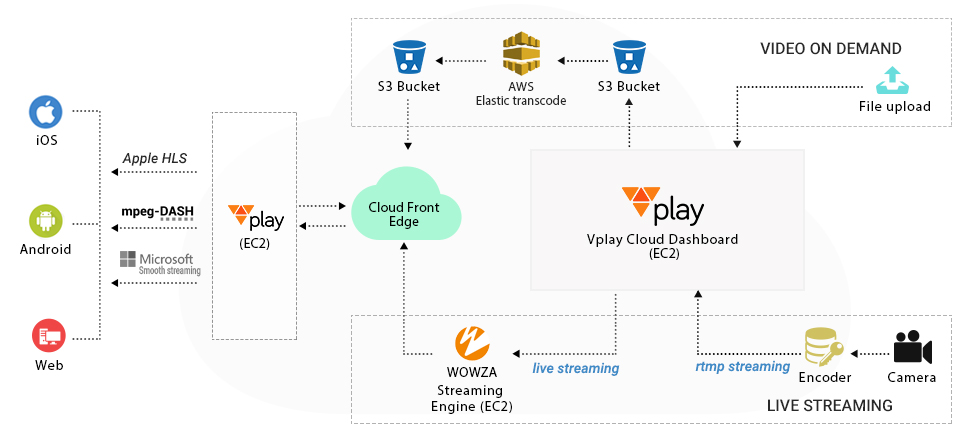
\includegraphics[width=16.5cm,height=10cm,keepaspectratio]{immagini/contus-vplay-cloud-architecture.jpg}
			\caption[Architettura di Contus Vplay]{Architettura di Contus Vplay
			\\
			Source: sito web di Contus Vplay \href{http://www.contus.com/video-on-demand-solution.php}{www.contus.com/video-on-demand-solution.php}}
		\end{center}
	\end{figure}
	Il servizio è predisposto per soddisfare le richieste dei clienti tramite tre protocolli, Apple HLS, MPEG-DASH e Microsoft Smooth Streaming, sulle principali piattaforme e con multiple qualità del video. La gestione dei contenuti avviene tramite una dashboard che viene mantenuta tramite una combinazione di server EC2 e il servizio CloudFront di \gls{AWS}. Oltre al sistema di streaming, Contus offre una serie di servizi allegati, come analisi sul traffico, profilazione, monetizzazione sugli annunci pubblicitari, cifratura delle connessioni e SDK per le maggiori piattaforme.

	\subsection{Streamroot}
	Streamroot offre un servizio di streaming ibrido. La sua particolarità rispetto alle altre soluzioni è quella di utilizzare un sistema di condivisione peer-to-peer dei contenuti scaricati dai clienti. In questo modo ciascun cliente non solo può contare sulla CDN che distribuisce i contenuti, ma anche su ogni altro utente che sta visualizzando gli stessi contenuti. Secondo i dati riportati dal servizio, questo tipo di distribuzione, unita al sistema di CDN, permette di abbassare il carico sui server di circa il 75\%. Streamroot viene utilizzato da molte aziende che hanno necessità di trasmettere ingenti quantità di dati, tra le quali Dailymotion, Eurosport e Canal+.

\section{Tecnologie utilizzate}
	\subsection{Linguaggi --- Java}
	Il linguaggio Java è stato scelto innanzitutto per la possibilità di eseguire il codice su qualsiasi piattaforma che offra una JVM;\@ in questo modo il sistema può essere eseguito su server con diversi sistemi operativi senza la necessità di riscriverne componenti o di essere ricompilato. Un altro vantaggio è quello di poter riutilizzare parte del codice scritto nel client Android, riducendone i tempi di sviluppo e aumentando la qualità del codice.

	\subsection{Piattaforma --- Apache Tomcat 8}
	Un servizio Java che espone dei WebSocket ha bisogno di una piattaforma che ne gestisca gli accessi ovvero un componente che implementi la classe JavaServer. Per questo progetto ho deciso di utilizzare Apache Tomcat 8 per il suo supporto nativo ai WebSocket. Inoltre, Tomcat 8 è il server Java open-source più diffuso, la sua documentazione è sufficiente chiara e completa e attualmente è l'unico a supportare completamente l'ultima versione di Java.

	\subsection{Tipo di dati scambiati --- JSON vs XML}
	Per poter inviare messaggi tramite un WebSocket è necessario definire una codifica. L'implementazione standard di Java permette di utilizzare stringhe di byte, stringhe di testo oppure di definire un codificatore e un decodificatore per gestire oggetti più complessi. Per semplificare lo sviluppo della piattaforma ho preferito utilizzare una codifica testuale, che mi permettesse di eseguire test automatici e manuali tramite client testuali. Le due codifiche maggiormente utilizzate che permettono di descrivere oggetti anche molto complessi sono JSON e XML.\@ Entrambe le codifiche soddisfano pienamente i requisiti necessari, ma JSON è molto meno prolisso di XML;\@ per questo motivo ho preferito tale linguaggio.

	\subsection{Strumenti di supporto}
		\subsubsection{Strumenti di codifica}
		Lo strumento che ho utilizzato per codificare ed eseguire i test sul sistema è stato l'IDE IntelliJ Idea, sviluppato da JetBrains, nella versione open-source ``Community Edition''. Questo editor, progettato appositamente per Java, è ricco di utili strumenti per velocizzare la codifica e l'analisi, come lo smart code completion, per i suggerimenti contestuali per il completamento del codice, i code template, per la rapida generazione di strutture di codice prestabilite, e sistemi di analisi e di automatizzazione dei task, come l'aggiornamento delle dipendenze o l'esecuzione dei test.

		\subsubsection{Strumenti di versionamento}
		Lo strumento di versionamento utilizzato durante il progetto è stato quello comunemente utilizzato dall'azienda, ovvero Git, con l'ausilio dei server di Bitbucket per l'automatizzazione di alcuni test.
		\\
		Il vantaggio di aver utilizzato Git durante lo sviluppo è stato quello di poter condividere velocemente le ultime modifiche con gli altri sviluppatori, pur mantenendo baseline sicure e testate.
		%TODO: estendere
		
		\subsubsection{Strumenti di test e verifica}
		Ho scelto di utilizzare il framework JUnit 4 per eseguire test di unità e di integrazione dopo un'attenta analisi delle sue funzionalità. Il sistema di test si è rivelato semplice ed efficace; mi ha permesso di realizzare test significativi con poco sforzo e ha contribuito alla buona qualità del codice. L'integrazione dell'IDE usato con JUnit permette anche di esportare i dati dei test, del coverage e delle analisi in formato HTML, facilmente consultabile anche senza strumenti di sviluppo dedicati. JUnit 4 è stato utile anche per eseguire benchmark per valutare l'efficacia del prodotto, tramite la realizzazione di una simulazione di conversazione tra un numero definito di utenti.
		
		\subsubsection{Strumenti di analisi di rete}
		Durante i test sulla sicurezza delle trasmissioni ho dovuto assicurarmi che il sistema inviasse contenuti sensibili non cifrati; per questo motivo ho avuto necessità di registrare le conversazioni tra alcuni utenti simulati. Per eseguire queste operazioni ho utilizzato Wireshark, un software open-source per l'analisi del traffico di rete. Wireshark permette di effettuare sniffing del traffico di rete, di visualizzare ciascun pacchetto e di filtrare facilmente i contenuti d'interesse. Tramite un'analisi eseguita con questo strumento ho potuto garantire che tutti i dati scambiati fossero cifrati end to end tramite TLS.\@
		
		\subsubsection{Strumenti di continuous integration}
		Per poter garantire l'indipendenza dalla piattaforma di sviluppo, in particolare durante l'esecuzione dei test, ho utilizzato un sistema \gls{Docker}. Questo strumento permette di configurare facilmente l'installazione e la configurazione di un software in sviluppo su una macchina virtuale minimale e di eseguire test e script su di essa. Tramite l'integrazione con Bitbucket ho potuto automatizzare queste attività, fornendo una maggiore qualità al codice senza dover svolgere compiti ripetitivi e onerosi in termini di tempo.
		\\
		Tramite le pipeline, il sistema di configurazione delle operazioni sui container \gls{Docker} di Bitbucket, ho potuto automatizzare anche il deploy dell'applicazione, limitando i tempi di manutenzione necessari al suo aggiornamento manuale.

\section{Nuovi orizzonti}
Tra gli obiettivi desiderabili indicati dall'azienda sono presenti lo studio di alcuni campi innovativi e la possibilità di utilizzarli nel contesto dello streaming video.

	\subsection{Blockchain}
	Blockchain è una tecnologia che permette di rendere delle informazioni pubbliche virtualmente impossibili da alterare. Il sistema si basa su catene di nodi distribuite in una rete peer-to-peer; ogni nodo contiene una certa quantità di informazioni fissata, un numero intero variabile, detto nonce, e l'hash dell'ultimo nodo della catena.
	\begin{figure}[H]
		\begin{center}
			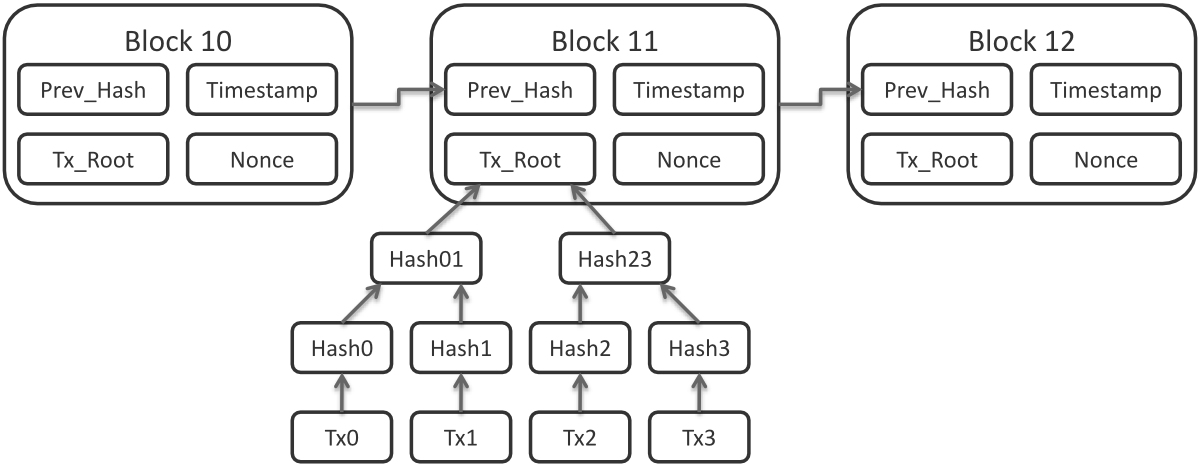
\includegraphics[width=16.5cm,keepaspectratio]{immagini/blockchain-data}
			\caption[Schema di funzionamento di una blockchain]{Schema di funzionamento di una blockchain
			\\
			Source: Wikimedia commons, Matthäus Wander, CC BY-SA 3.0}
		\end{center}
	\end{figure}
	Tutte le informazioni contenute nella catena sono pubblicamente accessibili e vengono condivise tra i client che sono connessi alla rete. La catena può essere estesa con nuovi nodi, ma affinché un nodo sia valido il suo hash deve soddisfare una regola nota a tutti i client. In generale questa impone che un certo numero di cifre in posizione fissata dell'hash siano uguali tra di loro e l'unico modo per far variare il risultato è cambiare il valore del numero intero all'interno dei dati. Dato che una funzione di hash è difficilmente reversibile, ovvero non è possibile ottenere i dati in input della funzione partendo dall'output, la complessità di questa operazione è molto alta e con l'aumentare del numero di cifre diventa sempre più difficile trovare un valore corretto. La regola della complessità varia in funzione del tempo necessario alla comunità di utenti per generare un nodo: con lo sviluppo di hardware in grado di eseguire le operazioni necessarie più velocemente, il sistema si adatterà rendendo più difficile la generazione. Quando un client riesce a generare un nodo adatto trasmette i valori adatti a dei server detti beacon, che accertano la correttezza del risultato e marcano l'istante temporale in cui il nodo è ritenuto valido, condividendo l'informazione a tutti i client vicini. Questi inizieranno a lavorare sul prossimo nodo della catena, mentre l'utente che ha scoperto il nodo ottiene dei vantaggi: ad esempio, nel caso di Bitcoin guadagna una ricompensa economica. In qualsiasi momento è possibile convalidare la creazione dei nodi precedenti applicando la funzione di hash su un nodo; inoltre tanto più la catena di nodi si allunga, tanto più è improbabile che qualcuno sia riuscito ad alterare l'intera sequenza, dato che questo richiederebbe l'aver trovato i valori corretti per generare ogni nodo in essa.
	\\
	La possibilità di rendere alcuni dati pubblici immodificabili può essere molto utile in molti campi, ma nel caso dello streaming affronta dei limiti molto importanti: mentre potrebbe essere possibile salvare interi file video all'interno di un singolo nodo, il throughput di questo metodo è molto basso a causa del tempo necessario al \engl{mining} del nuovo blocco. Si pensi che il tempo medio di generazione di un nodo di Bitcoin si aggira intorno agli otto minuti e trenta secondi. Un altro punto critico è il motivo che dovrebbe spingere gli utenti a eseguire le operazioni di hashing, ovvero la ricompensa: nel caso di un sistema di criptovaluta si può guadagnare denaro, ma parlando di streaming video non c'è una ricompensa ovvia. Una soluzione potrebbe essere quella di ottenere crediti per l'utilizzo del servizio, oppure un certo valore monetario; il problema di questo approccio è che potrebbe non essere autocontenuto nella sola piattaforma, limitandone l'efficacia e l'interesse. Esistono, inoltre, soluzioni meno onerose per la condivisione di file video su grande scala in modo decentralizzato, pur mantenendo la consistenza dei dati, come ad esempio il sistema Torrent, che permette di suddividere delle informazioni in blocchi cifrati univocamente identificati e di condividerli con chiunque ne faccia richiesta; in questo modo è comunque possibile garantire che il contenuto di ciascun blocco non sia stato alterato, senza necessità della complessità aggiunta da una blockchain.

	\subsection{Streaming peer to peer}
	Un nuovo sistema di distribuzione, particolarmente efficace se accoppiato ad una CDN, è quello di aggiungere al client una componente che permetta la condivisione dei chunk di video scaricati tramite una rete peer-to-peer. Gli utenti connessi diventano così parte della CDN migliorando aumentandone la portata in modo lineare seguendo la crescita della base di utenza.
	\\
	Esistono già soluzioni commerciali che adottano questo tipo di soluzione, ottenendo una grande riduzione del carico di rete sui server adibiti alla distribuzione e, di conseguenza, diminuendo i costi di gestione.
	\\
	Esistono anche soluzioni interamente peer-to-peer, come quella ideata dagli sviluppatori di WebTorrent\footnote{Sito web di WebTorrent: \href{https://webtorrent.io/}{webtorrent.io}}: il sistema sfrutta la rete BitTorrent e permette di condividere i contenuti man mano che vengono scaricati da altri utenti.
	\\
	Esistono anche soluzioni peer-to-peer per gli streaming real-time; una di queste è WebRTC:\@ tra le molteplici funzionalità dello standard è inclusa la possibilità di ritrasmettere i contenuti ricevuti agli altri utenti collegati allo stesso stream.

\section{Qualifica}
	\subsection{Verifica}
	la verifica di un prodotto è l'insieme delle operazioni atte a garantirne la qualità e il rispetto delle specifiche definite durante la progettazione. Può essere riassunto nella domanda ``\engl{did I build the system right?}''
		\subsubsection{Analisi statica}
		L'analisi statica consiste nei test che possono essere eseguiti sul prodotto senza compilare ed eseguire il codice. In questo tipo di test possiamo trovare, quindi, analisi grammaticali del codice, test su errori tipici, test sui file di configurazione, controlli sulla duplicazione del codice, ecc.
		\\
		L'analisi statica del prodotto è stata delegata ai test interni dell'IDE utilizzato, IntelliJ Idea. Questo esegue molti dei test sopra citati in modo automatico, mentre il codice viene scritto, fornendo utili suggerimenti.
		\\
		Una funzionalità che mi è sembrata particolarmente utile durante la verifica è il controllo automatico sulle classi importate: l'IDE controlla quali classi importate nel file vengono effettivamente utilizzate, segnala le mancanti offrendo suggerimenti e permette di eliminare quelle non necessarie.

		\subsubsection{Analisi dinamica}
		Con analisi dinamica si intendono le operazioni di controllo fatte sul codice compilato ed eseguito. Questi test includono asserzioni sullo stato dell'esecuzione ed esecuzioni controllate dei componenti, sia singolarmente, sia facendoli interagire l'uno con l'altro.
		\\
		Ho programmato l'analisi dinamica del prodotto durante l'analisi e la progettazione, per poi essere implementata durante la codifica. Ho realizzato i test di unità delle singole componenti e di integrazione, verificando che eseguissero i compiti assegnati dalle interfacce nel modo corretto, per poi passare ai test di sistema, eseguiti tramite simulazioni controllate.
		\\
		Un vantaggio importante nella scelta di eseguire test di sistema automatici è stata quella di poter valutare il prodotto nella sua interezza, generando un report chiaro sullo stato di sviluppo e sulle prestazioni ottenute. In particolare, dopo una prima fase di codifica ho scoperto un errore sulla gestione di alcuni task da parte del componente dedicato al reinvio dei messaggi proprio grazie a un test di questo tipo; alcuni messaggi non venivano inviati e le sessioni stabilite con i client venivano chiuse anticipatamente se il numero di utenti superava una certa soglia. La simulazione ha evidenziato questo problema e mi ha permesso di individuare e correggere il bug in poco tempo.

	\subsection{Validazione}
	La validazione di un prodotto consiste nel controllare che tutti i requisiti del prodotto vengano effettivamente soddisfatti e può essere riassunta nella domanda ``\engl{did I build the right system?}''
		\subsubsection{Validazione interna}
		Dato che il prodotto è destinato ad essere un componente di una più grande piattaforma, ancora in sviluppo, la validazione è stata interna. Il project manager e il mio tutor aziendale hanno eseguito tutti i test, le simulazioni e, come prova finale, hanno provato a comunicare tramite due client WebSocket.
